\documentclass[12pt]{article}
\textwidth 16.6cm
\textheight 22.6cm
\oddsidemargin 0cm

\usepackage{amssymb, amsmath, comment, graphicx, color}

% Title Page
\title{X-ray imaging}
\author{Do\u{g}a G\"{u}rsoy}

\begin{document}
\maketitle
\section{Physics of x-ray attenuation}
Let us assume a beam of X-rays passing through a medium and no scattered photons reach the collimated detector. Then, the intensity of X-rays emerging from the medium along the incident direction is given by:
\begin{equation}
 I(\textbf{r},w) = I_0(w)\exp\left(-\frac{1}{2}\int\mu(\textbf{r},w)dl\right),
 \label{intensity}
\end{equation}
where $I_o(w)$ is the incident intensity of X-rays and $\mu(\textbf{r},w)$ denotes the total attenuation within the medium. Here, $w\in[0,\infty)$~[1/s] and $\textbf{r}\in\mathcal{R}^3$~[cm] represent the frequency and spatial dependencies of the underlying functions at the detector site. Considering the medically relevant energy bandwidth of 20 to 120~keV, the photoelectric absorption and incoherent scattering are the primary interaction mechanisms of X-rays with the materials. So the projected attenuation can be decomposed into two parts as follows:
\begin{equation}
 \mu(\textbf{r},w) = \mu_{a}(\textbf{r},w)+\mu_{s}(\textbf{r},w)
 \label{attenuation}
\end{equation}
with $\mu_{a}(\textbf{r},w)$ and $\mu_{s}(\textbf{r},w)$ being the absorption and scattering contributions to the total x-ray attenuation, respectively. The photoelectric absorption and incoherent scatterings can be modeled by:
\begin{eqnarray}
 \mu_a(\textbf{r},w) &=& R\left\lbrace\sum_m N_m(\textbf{x})\sigma_{\mu,i,m}(w)\right\rbrace \label{absorption} \\
 \mu_s(\textbf{r},w) &=& R\left\lbrace\sum_m N_m(\textbf{x})\sigma_{c,a,m}(w)\right\rbrace, \label{scattering}
\end{eqnarray}
where $R\left\lbrace.\right\rbrace$ represents the Radon transform in spatial coordinates. $m$ is the element index (representing the elements within the object). $\sigma_{\mu,i,m}(w)=2r_e\lambda(w)f_{i,m}(w)$~[cm$^2$] is defined as the cross-section for photoelectric emission of the element. $f_{i,m}(w)$ is the imaginary part of the atomic form factor of the corresponding element. $\lambda(w)$~[cm] is the wavelength of the x-ray beam. $r_e\approx2.8e-13$~[cm] is the classical electron radius. $N(\textbf{x})=W(\textbf{x})\rho_{T}(\textbf{x})N_A/A_r$~[1/cm$^3$] is the the number of atoms of elements per unit volume at location $\textbf{x}$ within the medium where $W(\textbf{x})\in[0,1]$ is the mass weighting factor of the element. $\rho_{T}(\textbf{x})$~[g/cm$^3$] is the density distribution of the medium, $A_r$~[g/mol] is the atomic weight of the element and $N_A\approx6.02e+23$~[1/mol] is the Avagadro constant. $\sigma_{c,a,m}(w)=Z_m\sigma_{c,e}(w)$ is the Compton cross-section of the atom with $Z$ being the atomic number of the corresponding element and $\sigma_{c,e}(w)$ being the Compton cross-section of the electron. $\sigma_{c,e}(w)$ is modeled based on the Klein-Nishina equation:
\begin{multline}
 \sigma_{c,e}(w) = 2\pi r_e^2\left[\left(\frac{1+\xi(w)}{\xi(w)^2}\right) \left(\frac{2(1+\xi(w))}{1+2\xi(w)^2}-\frac{\ln(1+2\xi(w))}{\xi(w)}\right)\right. \\
 \left.\left.\frac{\ln(1+2\xi(w))}{\xi(w)}\right) + \frac{\ln(1+2\xi(w))}{2\xi(w)}-\frac{1+3\xi(w)}{(1+2\xi(w))^2}\right],
\end{multline}
where $\xi(w)=\eta\hbar w/(m_ec^2)$ is the energy ratio of the incident x-ray and the electron energy. $\hbar\approx6.5e-19$~[keV/s] is the reduced Planck constant. $w$~[1/s] is the angular freqeuncy of x-ray. $\eta\approx1.6e-9$ is the necessary transformation factor to convert the SI-unit keV to cgs-unit erg (i.e., 1~keV is equal to $1.6e-9$~ergs). $m_e\approx9.1e-28$~[g] is the electron rest mass. $c\approx3e+6$~[cm/s] is the speed of light in the vacuum.

\subsection{A model for photoelectric cross-section}
When the photon energy is well above an absorption edge but the energy of the emitted
electron is not relativistic the cross-section of photoelectric emission is usually modeled as:
\begin{equation} 
 \sigma_{\mu,i,m}(w) = KZ^5_m\xi^{-3.5}(w) \label{photo1}
\end{equation}
with $K=4\sqrt{2}\alpha^4\sigma_T$~[cm$^2$] being an area constant where $\alpha=e/\hbar c$ and $\sigma_T=8\pi r_e^2/3$~[cm$^2$] are respectively the fine structure constant and the Thompson cross-section of the electron. This is the result obtained theoretically using the plane-wave Born approximation. Expression~\ref{photo1} approximates: $\sigma_{\mu,i,m}(w) = 2r_e\lambda(w)f_i(w)$, where $f_i(w)$ is the imaginary part of the atomic factor of the element. To give an example, the corresponding plots for the elements H, C, O and N are presented in figure~\ref{validity1}. The top row corresponds to the spetra of 0.1--100~keV. It is clearly visible that the approximation is valid as the energy of the x-ray is increased. The bottom row corresponds to the spectra of 20--100~keV which is the feasible range for medical applications. In this frequency range, the relative approximation error is around 1 about 20~keV and about 0.3 for 100~keV. Due to the high relative errors at the desired frequency band of 20--100~keV, the model is redefined by introducing a correction variable $a$ for each element as follows: $
 \hat\sigma_{\mu,i,m}(w) = KZ^5_m\xi^{-a_m}(w)$. For the aforementioned elements the corresponding correction terms for the desired frequency band is calculated to be: $a_H=3.25$, $a_C=3.35$, $a_O=3.30$ and $a_N=3.32$. The corresponding plots of the cross-section after correction is given on figure~\ref{validity2}.
\begin{figure}
\centering
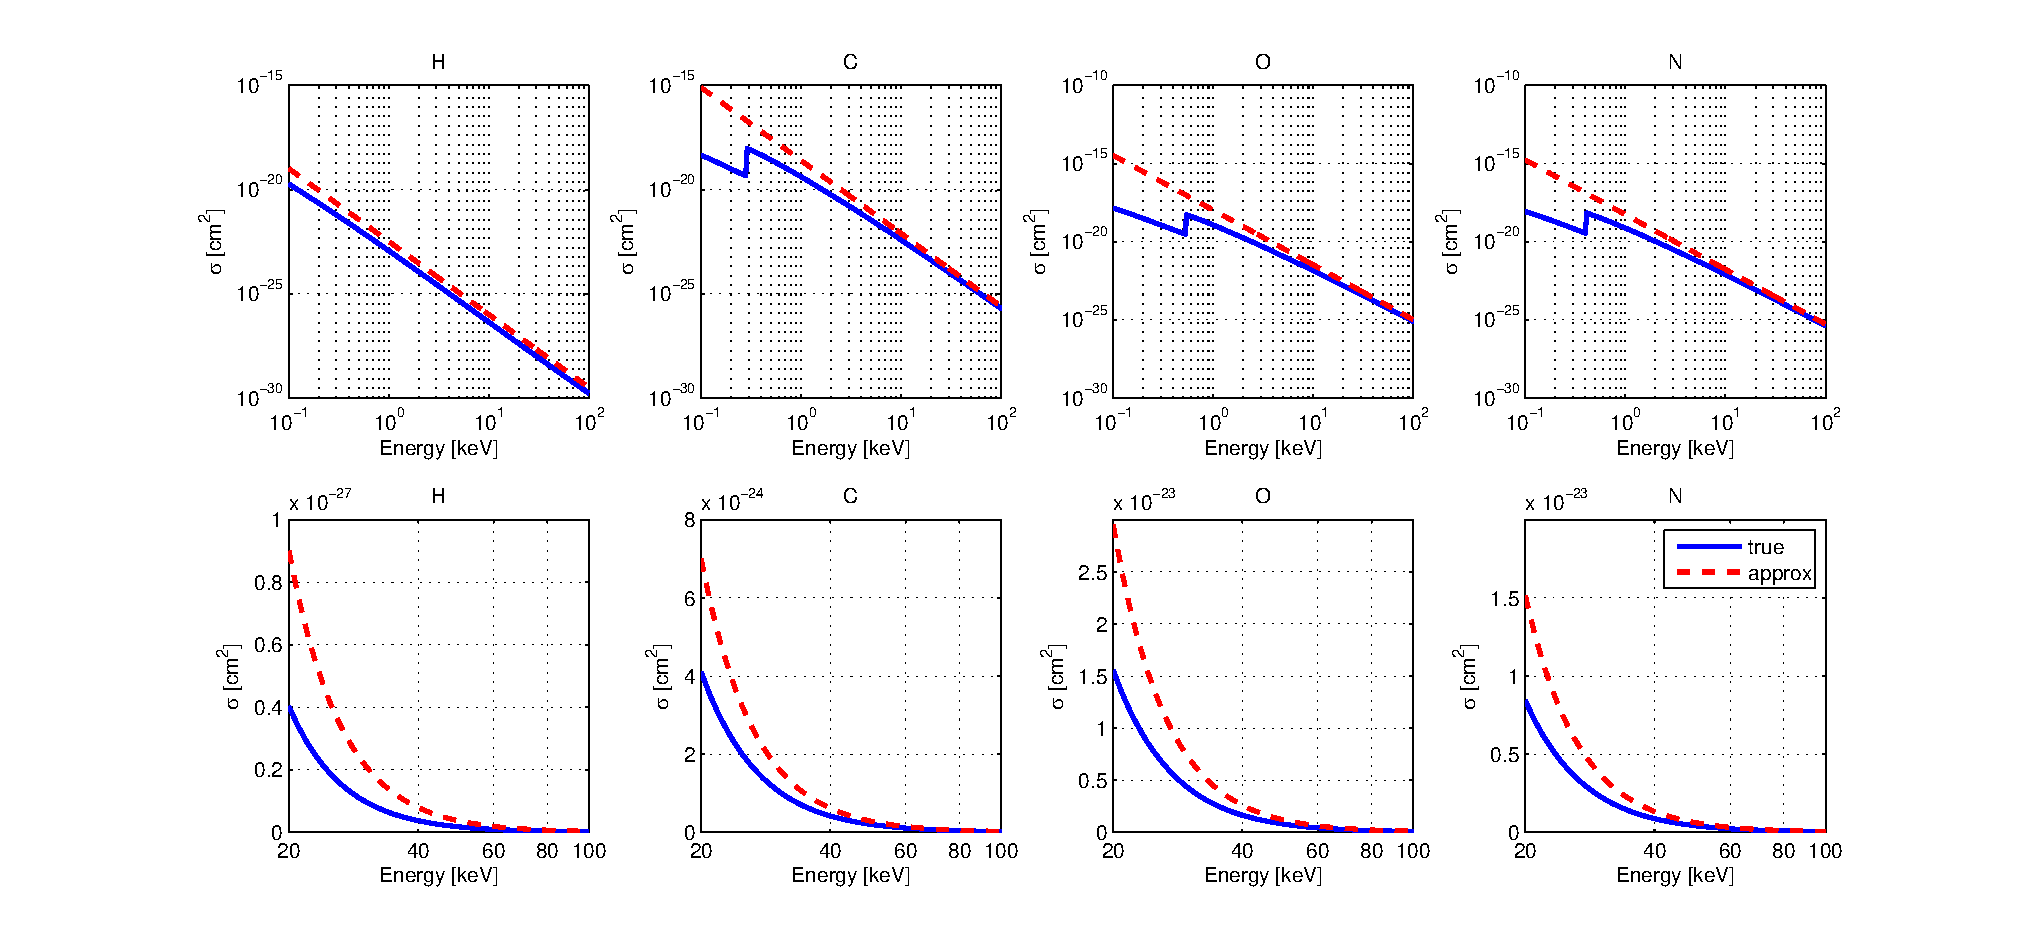
\includegraphics[width=1\textwidth]{imgs/validity1.eps}
\caption{Comparison of the true and approximated spectra of the cross-sections for the photoelectric absorption after correction. The top row corresponds to the spetra of 0.1--100~keV and the bottom row corresponds to the spectra of 20--100~keV.}
\label{validity1}
\end{figure}
\begin{figure}
\centering
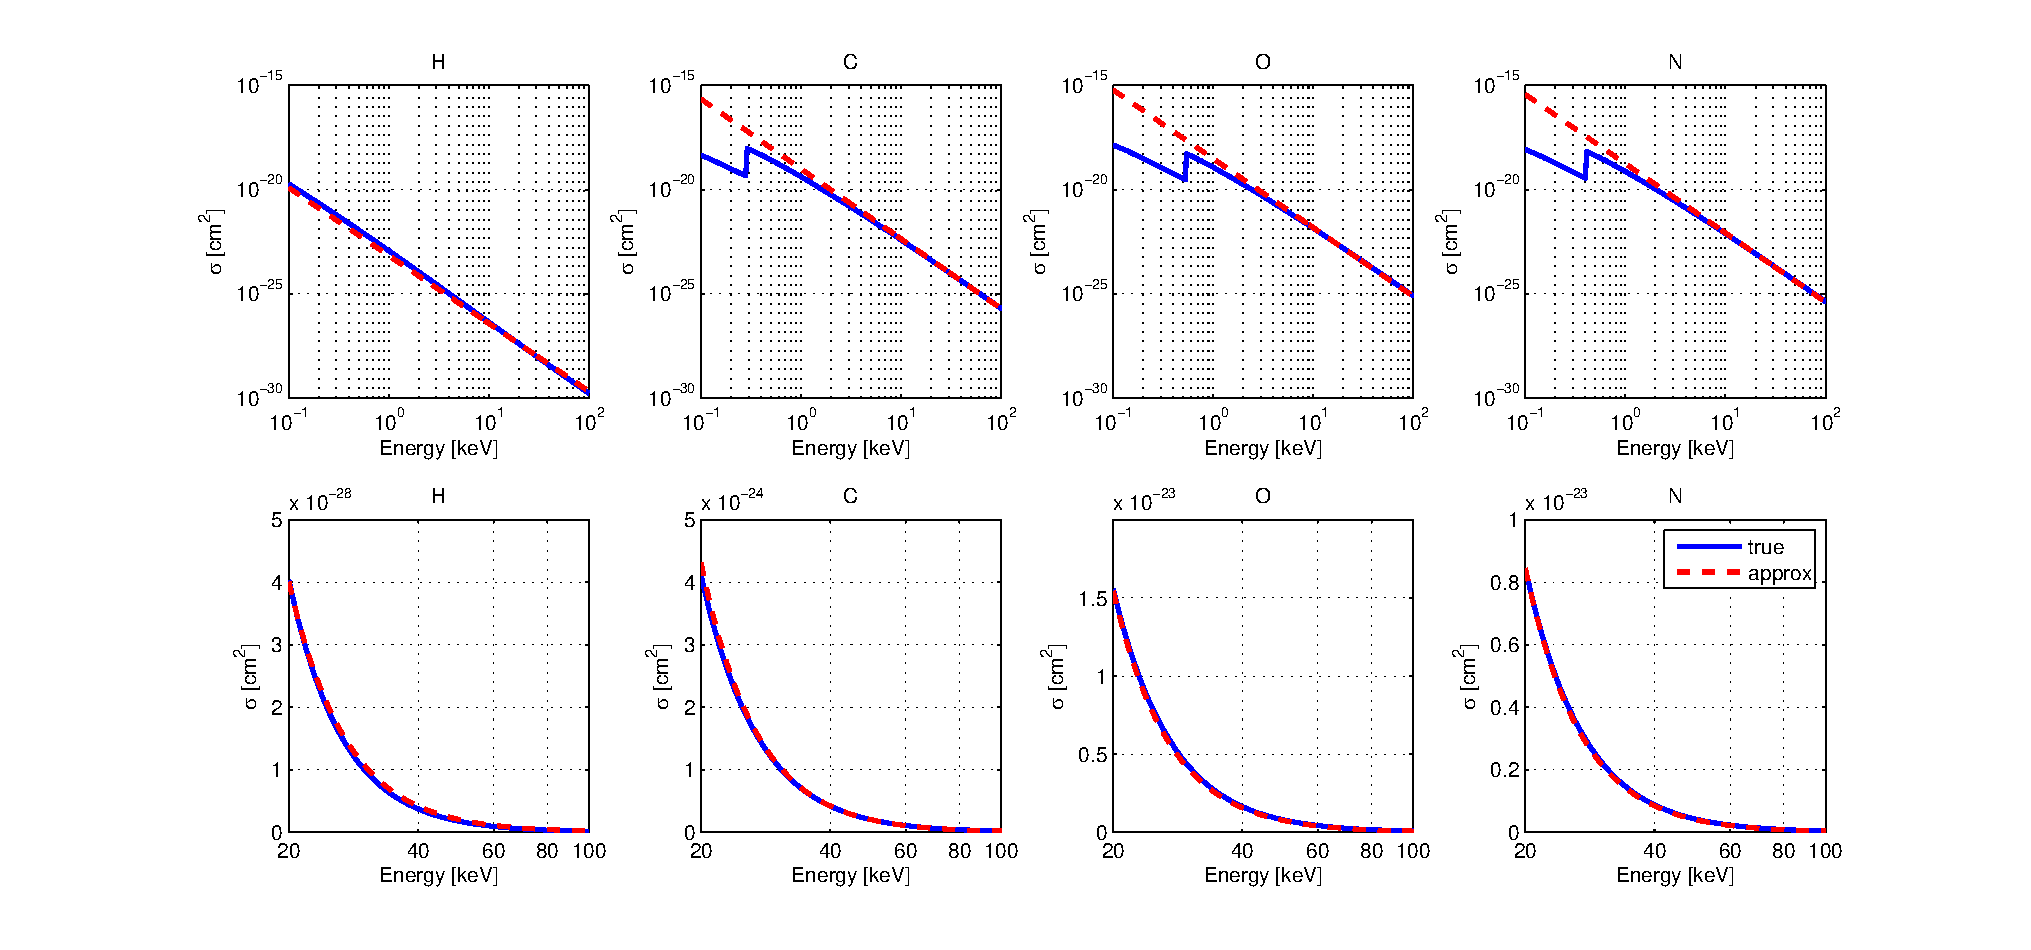
\includegraphics[width=1\textwidth]{imgs/validity2.eps}
\caption{Comparison of the true and approximated spectra of the cross-sections for the photoelectric absorption. The correction terms are $a_H=3.25$, $a_C=3.35$, $a_O=3.30$ and $a_N=3.32$ The top row corresponds to the spetra of 0.1--100~keV and the bottom row corresponds to the spectra of 20--100~keV.}
\label{validity2}
\end{figure}

\subsection{Recovery of electron density from attenuation}
By substituting equation~\ref{absorption} and \ref{scattering} into equation~\ref{attenuation} and taking the inverse Radon transform (i.e., $\mu(\textbf{x},w)=R^{-1}\left\lbrace\mu(\textbf{r},w)\right\rbrace$), the attenuation coefficient distribution within the medium is given as:
\begin{equation}
 \mu(\textbf{x},w) = \sum_m N_m(\textbf{x})\sigma_{\mu,i,m}(w) + \sum_m N_m(\textbf{x})\sigma_{c,a,m}(w). \label{mu}
\end{equation}
Also assuming that the atomic number represents the number of electrons in the atom, we can use the relationship: $\sigma_{c,a,m}(w)=Z_m\sigma_{c,e}(w)$ and $\rho_{e,m}(\textbf{x})=N_m(\textbf{x})Z_m$ (defined as electron density) to end up with the following expression for the attenuation:
\begin{equation}
 \mu(\textbf{x},w) = \sum_m \left[\rho_{e,m}(\textbf{x})\left(KZ^4_m\xi^{-3.5}(w) + \sigma_{c,e}(w)\right)\right].
\end{equation}
This is a quite usefull equation because the spatial and frequency dependencies of the attenuation can be decomposed. The above expression is simply a linear equation such that when the attenuation at different x-ray energies is known (e.g., from inverse tomography), the electron density can be retrieved by a simple inversion.

\subsection{Defining the reconstruction problem for electron density}
Let us formalize the inverse problem mentioned in the last section. By defining $n$ as the number of frequency sampling, $m$ as the number of elements in the medium and $p$ is the position index, the solution for $\rho_{e,m}(\textbf{x})$ can be acquired by solving the following linear equation:
\begin{equation}
  \textbf{A}\textbf{q} = \textbf{B}, \label{axb}
\end{equation}
where $\textbf{A}\in\mathcal{R}^{n\times m}$, $\textbf{q}\in\mathcal{R}^{m\times p}$ and $\textbf{B}\in\mathcal{R}^{n\times p}$ are the matrices with the following coefficients,
\begin{eqnarray}
 a_{m,n} &=&  KZ^4_m\xi^{-a_m}(w_n) + \sigma_{c,e}(w_n) \\
 q_{n,p} &=& \rho_{e,n}(x_p) \\
 b_{n,p} &=& \mu(x_p,w_n).
\end{eqnarray}
Thus, it is required to have at least $m$ measurements at different frequencies for a unique solution. There are countless ways to solve the problem (depending on what kind of solution you prefer), but the common option would be solving the following minimization problem:
\begin{equation}
  \arg\min_\textbf{q}\left\lbrace \mathcal{F}:\frac{1}{2}\left|\left|\textbf{A}\textbf{q} - \textbf{B}\right|\right|^2_2+\frac{\lambda}{2}\left|\left|\textbf{R}\textbf{q}\right|\right|^2_2\right\rbrace,
\end{equation}
where $\lambda$ and $\textbf{R}$ are the regularization parameter and regularization matrix respectively. 

\subsection{Effective values}
It is easier to solve for the effective (or total) electron density rather than solving for the electron densities for each element within the object. In that case we define: $\rho_e=\sum_m\rho_{e,m}$. Expression~8 can be written as:
\begin{equation}
 \mu(\textbf{x},w) = \rho_e(\textbf{x})\left(KZ^4_{eff}\xi^{-3.5}(w) + \sigma_{c,e}(w)\right).
\end{equation}
Note that the atomic number is replaced by the ``effective atomic number'' which is also unknown. So the degrees of freedom is reduced to two (total electron density and effective atomic number). This approach has been adopted in many multi-energy decomposition methods.

\section{Relationship between Compton scattering and photoelectric absorption}
\begin{figure}
\centering
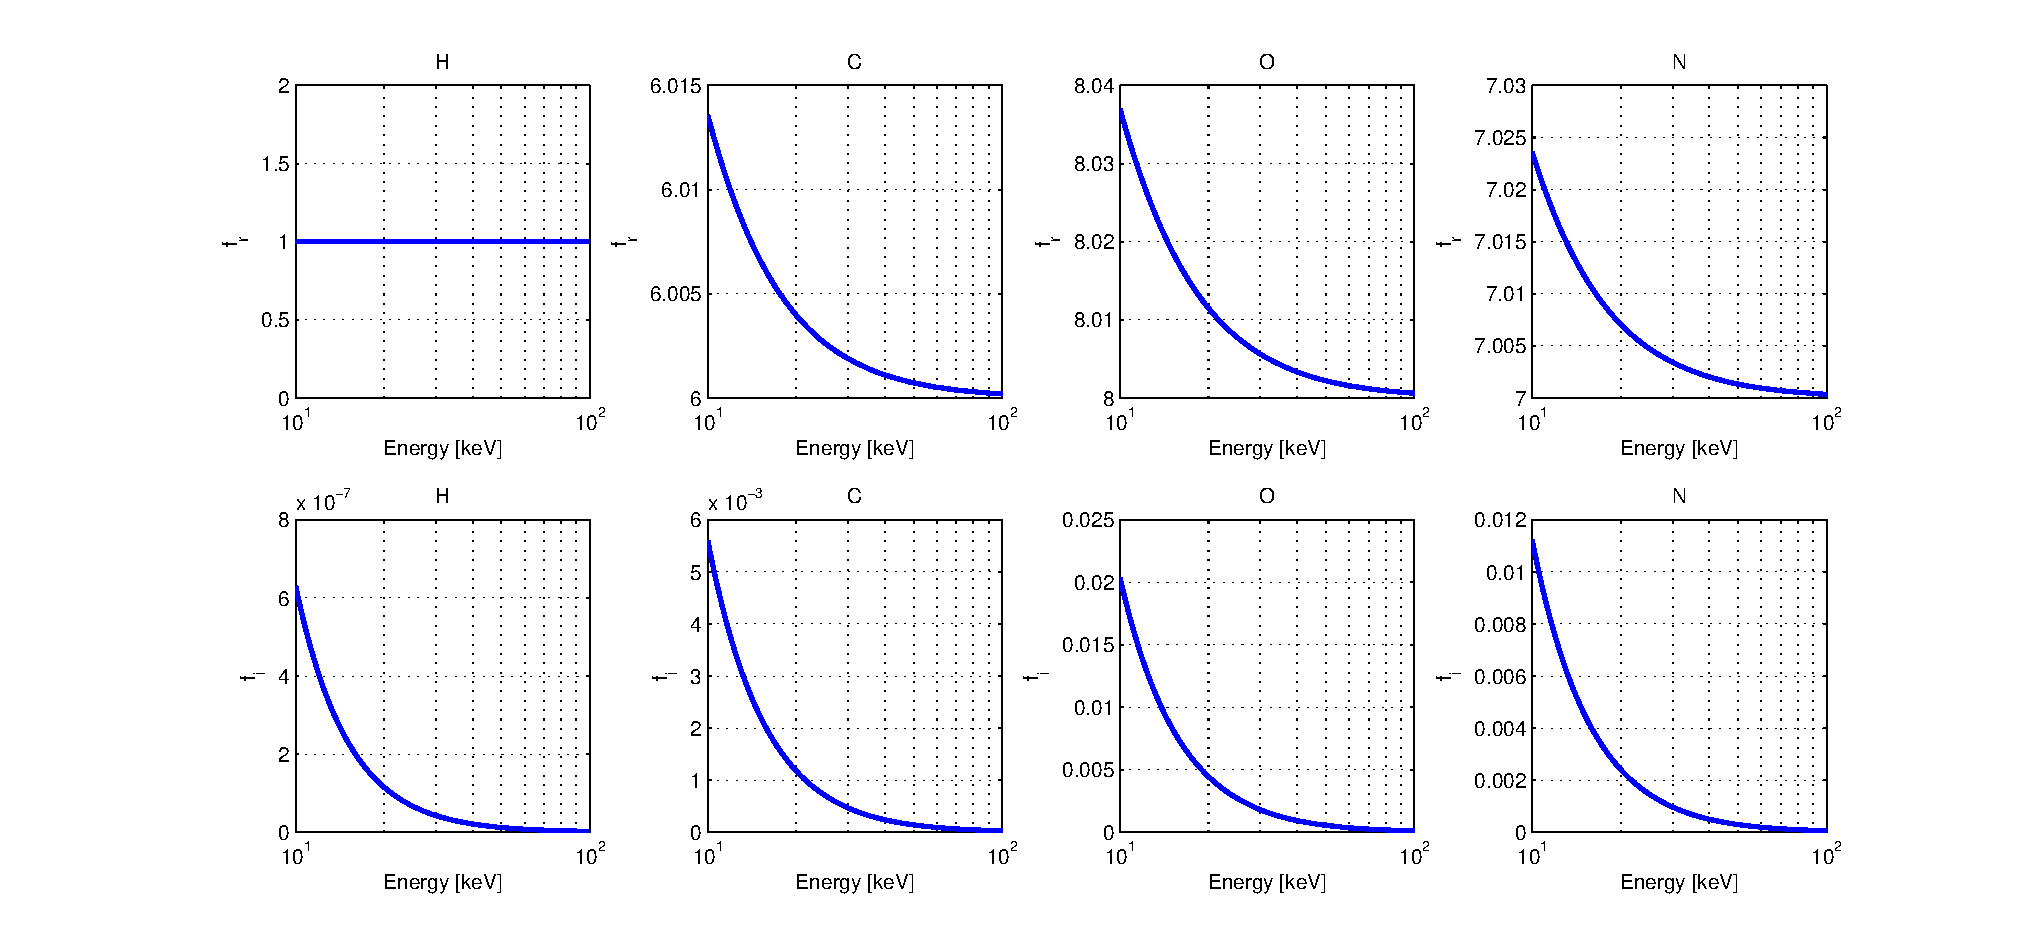
\includegraphics[width=1\textwidth]{imgs/formFactorsHCON.eps}
\caption{Atomic form factors of the elements: H, C, O and N between the energy range 20--120~keV (imported from NIST database). Top and bottom rows represent the $f_r$ and $f_i$, respectively. Note that $f_r$ values at this frequency range are close to the atomic number of the corresponding elements. Thus, in many cases $\sum_i N_if_{r,i}\approx\sum_i N_iZ_i$ is considered as the electron density within that energy window.}
\label{formFactorsHCON}
\end{figure}

Let us remember that the refractive index can as well be represented in terms of the atomic form factors as follows:
\begin{equation}
 n(\textbf{x},w) = 1-\frac{r_e\lambda^2(w)}{2\pi}\sum_m N_m(\textbf{x})f_m(w),
 \label{formfactor}
\end{equation}
where $m$ is the element index and $f(w)=f_r(w)-jf_i(w)$ is the complex energy dependent function, the real and imaginary parts of which are called the atomic form factors (see figure~\ref{formFactorsHCON} for some examples):
\begin{eqnarray}
 \delta(\textbf{x},w) &=& \frac{r_e\lambda^2(w)}{2\pi}\sum_m N_m(\textbf{x})f_{r,m}(w),
 \label{delta}\\
 \beta(\textbf{x},w) &=& \frac{r_e\lambda^2(w)}{2\pi}\sum_m N_m(\textbf{x})f_{i,m}(w).
 \label{beta}
\end{eqnarray}
$N(\textbf{x})$~[1/cm$^3$] is the the number of atoms of elements per unit volume at location $\textbf{x}$ within the medium:
\begin{equation}
 N(\textbf{x})=W(\textbf{x})\frac{N_A}{A_r}\rho_{T},
\end{equation} 
where $W(\textbf{x})\in[0,1]$ is the mass weighting factor of the element, $\rho_{T}$~[g/cm$^3$] is the total density of the medium, $A_r$~[g/mol] is the atomic weight of the element and $N_A\approx6.02e+23$~[1/mol] is the Avagadro constant. In fact, the real and imaginary parts of the refractive index (equivalently we can dare to say the absorption and scattering) are related and can be modeled using the Kramers-Kronig relations as follows:
\begin{eqnarray}
 \delta(\textbf{x},w) &=& 1-\frac{2}{\pi}\mathrm{P} \int_0^\infty\frac{w'\beta(\textbf{x},w')}{w'^2-w^2}dw', \label{kk1}\\
 \beta(\textbf{x},w) &=& \frac{2w}{\pi}\mathrm{P} \int_0^\infty\frac{\delta(\textbf{x},w')-1}{w'^2-w^2}dw'.
 \label{kk2}
\end{eqnarray}
where $\mathrm{P}$ denotes the principal value of the integral. $\delta(\textbf{x},w)$ and $\beta(\textbf{x},w)$ are the refractive index decrement and extinction coefficient respectively. It can be transformed into the object domain as:
\begin{equation}
 \mu(\textbf{x},w) = R^{-1}\left\lbrace-2\ln\left(\sqrt{P(\textbf{r},w)}\right)\right\rbrace,
 \label{mu1}
\end{equation}
where, $\mu(\textbf{x},w)\in[0,\infty)$~[1/cm] is defined as the attenuation coefficient of the medium and $P(\textbf{r},w)$ is the measured power spectrum of x-rays. So after several substitutions one can write an expression equivalent to expression~7:
\begin{equation}
 \mu(\textbf{x},w) = \frac{4\pi}{\lambda(w)}\beta(\textbf{x},w)+\sum_m N_m(\textbf{x})\sigma_{c,a}(w).
 \label{mu2}
\end{equation}
Recall that $\sigma_{c,a}(w)=Z\sigma_{c,e}(w)$, thus, equation~\ref{mu2} can be written as:
\begin{equation}
  \mu(\textbf{x},w) = \frac{4\pi}{\lambda(w)}\beta(\textbf{x},w)+\sigma_{c,e}(w)\rho_e(\textbf{x}),
 \label{mu3}
\end{equation}
Note that $\sigma_{c,e}(w)$ is the Compton cross-section of the electron and is independent of the atom type. In the 20--120~keV range, the real part of the atomic form factors can be approximated with the corresponding atomic number of the elements (i.e., $\delta(\textbf{x},w) \approx r_e\lambda^2(w)\rho_e(\textbf{x})/2\pi$). Thus, equation~\ref{mu3}, can be approximated by:
\begin{equation}
 \mu(\textbf{x},w) = \frac{4\pi}{\lambda(w)}\beta(\textbf{x},w) +\frac{2\pi\sigma_{c,e}(w)}{r_e\lambda^2(w)}\delta(\textbf{x},w).
 \label{muTotal}
\end{equation}
Equation~\ref{muTotal} presents the relationship between the real and imaginary parts of the refraction index in $\mu(\textbf{x},w)$. The first and second terms at the right hand side refer to as the attenuations due to absorption and scattering, respectively.

\subsection{Retrieval of $\beta$}
By combining equation~\ref{muTotal} with the Kramers-Kronig relation as given by equation~\ref{kk1}, $\beta(\textbf{x},w)$ can be decoupled from $\delta(\textbf{x},w)$ as follows:
\begin{equation}
 \mu(\textbf{x},w) = \frac{4\pi}{\lambda(w)}\beta(\textbf{x},w) +\frac{2\pi\sigma_{c,e}(w)}{r_e\lambda^2(w)}\left(1-\frac{2}{\pi}\mathrm{P} \int_0^\infty\frac{w'\beta(\textbf{x},w')}{w'^2-w^2}dw'\right) \label{beta1}
\end{equation}
The integral equations~\ref{beta1} can be treated according to the Fredholm theory. After rearrangements, equation~\ref{beta1} can be rearranged in the form of a singular integral equation of the second kind with a Cauchy kernel as follows:
\begin{equation}
 \beta(\textbf{x},w) = f_\beta(\textbf{x},w) + \mathrm{P}\frac{1}{\pi}\int_0^\infty\frac{\kappa_\beta(w,w')}{w'-w}\beta(\textbf{x},w')dw'
\end{equation}
where $f_\beta(\textbf{x},w)$ is the known function and $\kappa_\beta(w,w')$ is the auxiliary function defined as follows:
\begin{eqnarray}
 f_\beta(\textbf{x},w) &=& \left(\frac{\lambda(w)}{4\pi}\mu(\textbf{x},w)-\frac{1}{2}\psi^{-1}(w)\right) \\
 \kappa_\beta(w,w') &=& \psi^{-1}(w)\left( \frac{w'}{w'+w}\right).
\end{eqnarray}
In here, $\psi(w)=r_e\lambda(w)/\sigma_{c,e}(w)$.

\subsection{Retrieval of $\delta$}
By combining equation~\ref{muTotal} with the dual Kramers-Kronig relation as given by equation~ \ref{kk2}, $\delta(\textbf{x},w)$ can be written as:
\begin{equation}
 \mu(\textbf{x},w) = \frac{8w}{\lambda(w)}\mathrm{P} \int_0^\infty\frac{\delta(\textbf{x},w')-1}{w'^2-w^2}dw' +\frac{2\pi\sigma_{c,e}(w)}{r_e\lambda^2(w)}\delta(\textbf{x},w).
 \label{delta1}
\end{equation}
After rearrangements of equation~\ref{delta1}, one can write in the form of integral equation of second kind:
\begin{equation}
 \delta(\textbf{x},w) = f_\delta(\textbf{x},w) + \mathrm{P}\frac{1}{\pi}\int_0^\infty\frac{\kappa_\delta(w,w')}{w'-w}\beta(\textbf{x},w')dw',
\end{equation}
where $f_\delta(\textbf{x},w)$ and $\kappa_\delta(w,w')$ are as given:
\begin{eqnarray}
 f_\delta(\textbf{x},w) &=& 2\psi(w)\left(  \frac{\lambda(w)}{4\pi}\mu(\textbf{x},w) + 1 \right) \\
 \kappa_\delta(w,w') &=& -4\psi(w)\left( \frac{w}{w'+w} \right).
\end{eqnarray}

\section{Transport of intensity}
As x-rays (having some degree of coherence) propagate the wavefront evolves according to the variations in the phase distribution of the x-rays. This is best modeled by the following differential equation:
\begin{equation}
 -k\frac{\partial I(\textbf{r},w)}{\partial l}=\nabla\cdot\left(I(\textbf{r},w)\nabla\phi(\textbf{r},w)\right)
\end{equation}
with $\phi(\textbf{r},w)$ as the phase of x-rays. The left hand side is the directional rate of change of x-ray intensity in propagation direction and $\nabla$ is the gradient operator defined on the plane orthogonal to the propagation direction. Note that phase can be related with the electron density as follows:
\begin{equation}
 \phi(\textbf{r},w) = -\lambda r_e\int\rho_e(\textbf{x},w)d^3x
\end{equation}
The refraction of x-rays is very tiny (i.e., the real part of the refractive index is almost one). So the rate of change of intensity in propagation direction can be linearly approximated using: $(I_2(\textbf{r},w)-I_1(\textbf{r},w))/D$. $I_1(w)$ and $I_2(w)$, are the measurements at two different detector distances with respect to the object and $D$ is the distance between them. Then, we can write the transport of intensity expression as follows (Wilkins, Yan, etc.):
\begin{eqnarray}
 I_2(\textbf{r},w) &=& I_1(\textbf{r},w)\left(1 +D\frac{\lambda^2r_e}{2\pi}\nabla^2P(\textbf{r})\right)  +D\frac{\lambda^2r_e}{2\pi}I_1(\textbf{r},w) \cdot\nabla P(\textbf{r})\nonumber
\label{eqn:tie_complete}
\end{eqnarray}
where $P(\textbf{r})=\int\rho_e(\textbf{x},w)d^3x$ is the projected electron densities. Note that $P$ is assumed to be independent of x-ray energy.

\subsection{Numerical tests on approximations}
One of the best ways to perform numerical tests is using a 2-D circular object that can be modeled analytically. The analytical expressions for the projection for a circular object is given:
\begin{equation}
 F(r) = 2q(a^2-r^2)^{1/2},
\label{eqn:proj}
\end{equation}
where $a$ is the radius of the circle, $r$ is the coordinates in projection domain and $q$ is the material property (can be attenuation, electron density, etc.). Thus when we plug that into TIE equation, we get,
\begin{eqnarray}
I_2(\textbf{r},w)&=& I_{0}(w)\exp\left[-2\mu(a^2-r^2)^{1/2}\right]\left[1 -D\frac{2\lambda^2r_er^2\rho_e}{2\pi(a^2-r^2)^{3/2}}\right] \\
&& +D\frac{\lambda^2r_e}{2\pi}I_{0}(w)\left(\frac{2r}{\exp\left(2(a^2-r^2)^{1/2}\right)(a^2-r^2)^{1/2}}\right)\cdot \left(\frac{-2r\rho_e}{(a^2-r^2)^{1/2}}\right)\nonumber
\end{eqnarray}
where $\mu$ and $\rho_e$ are respectively introduced as the attenuation coefficient and the electron density of the object. By using that relation one can test the contribution of different terms in TIE equation.  For a wide variety of materials the last term on the right hand side can be dropped. Let us make a first order approximation to the exponential function:
\begin{equation}
  I_2(\textbf{r},w) = I_{0}(w)\left[1-\int\mu(\textbf{x},w)d^3x -D\frac{\lambda^2r_e}{2\pi}\nabla^2P(\textbf{r})\right]
 \label{approx}
\end{equation}

\subsection{Elemental decomposition}
By putting the line integral of attenuation coefficients, expression~\ref{approx} can be arranged as:
\begin{eqnarray}
\frac{I_2(\textbf{r},w)}{I_{0}(w)}-1 &=&  \sum_m \left( KZ_m^4E^{-a}(w)+\sigma_{\text{KN}}(w) +D\frac{\lambda^2r_e}{2\pi}\nabla^2\right)P_m(\textbf{r})
%&=& I_{0}(w)\left[1-\frac{1}{2}\int\rho_{e}(\textbf{x})KZ^4(\textbf{x})E^{-a}(w)d^3x +  \left( \frac{1}{2}\sigma_{\text{KN}}(w)-D\frac{\lambda^2r_e}{2\pi}\nabla^2\right) P(\textbf{r})\right]
\end{eqnarray}
A unique solution can be obtained assuming at least $m$ different equations, i.e., different energies. 

\subsection{Material decomposition}
Similiarly, one can write:
\begin{equation}
 \frac{I_2(\textbf{r},w)}{I_{0}(w)}-1  = KE^{-a}(w)A_1(\textbf{r})+\left( \sigma_{\text{KN}}(w)+D\frac{\lambda^2r_e}{2\pi}\nabla^2\right)A_2(\textbf{r})
\end{equation}
where, $A_1(\textbf{u})$ and $A_2(\textbf{u})$ are used for brewity and they are given as:
\begin{eqnarray}
 A_1(\textbf{u}) &=& \mathcal{F}\left\lbrace \int\rho_{e}(\textbf{x})Z^4(\textbf{x})d^3x \right\rbrace \\
 A_2(\textbf{u}) &=& \mathcal{F}\left\lbrace P(\textbf{r})\right\rbrace
\end{eqnarray}
At least two equations are needed to solve the above problem.

 \begin{thebibliography}{1}

  \bibitem{} Gureyev T, Roberts A and Nugent, Partially coherent fields, the transport-of-intensity equation, and phase uniqueness {\em JOSA-A} 1995

  \bibitem{} Gureyev and Nugent Phase retrieval with the transport-of-intensity equation. II. Orthogonal series solution for nonuniform illumination {\em JOSA-A} 1996 

  \bibitem{} Gureyev, Roberts and Nugent, Phase retrieval with thransport-of-intensity equation: matrix solution with use of Zernike polynomials {\em JOSA-A} 1995 

  \bibitem{} Gureyev, Paganin, Myers, Ya, Nesterets and Wilkins, Phase and amplitude computer tomography {\em APL} 2006 

  \bibitem{} Arhatarim Hannah, Balaur abd Peele, Phase imaging using a polychromatic x-ray lab source {\em Opt. Exp.} 2008 

  \bibitem{} Arhatari, Riessen and Peele, Polychromatic x-ray tomography: direct quantitative phase reconstruction {\em Opt Exp} 2012 

  \bibitem{} Teague, Irradiance moments: their propagation and use for unique retrieval of phase {\em JOSA} 1982

  \bibitem{} Teague, Deterministic phase retrieval: a Green's function solution {\em JOSA} 1983

  \bibitem{} Wu and Liu, Phase-space formulation for phase-contrast x-ray imaging {\em Applied Optics} 2005
 

  \end{thebibliography}


\end{document}












